\documentclass[A4]{article}

%\usepackage[iso]{umlaute}
%\usepackage{german}
\usepackage{graphicx}
\setlength{\parindent}{0cm}
\setlength{\columnsep}{25pt}
\sloppy

% Your name
\author{Johnny Walker \\ Technische Universit\"at M\"unchen}

\title{Seminar Advanced Computer Architecture \\
       {\bf Your Paper Title}
}

% Date of your talk
\date{2.4.2042}


\begin{document}

\maketitle

\begin{abstract}

This abstract should contain a short summary of what this
article is about. That is, a short introduction into the
topic, the main issues discussed, any why this is interesting.
Finally, some very short conclusion/results of the discussed
ideas. From this, the reader should be able to estimate whether
it is worth to read on.
\end{abstract}

% \section defines numbered parts of the paper with titles
% there also are \subsection and \subsubsection
\section{Introduction}

% Use labels to be able to refer to this position from somewhere else
\label{introduction}

The introduction of a scientific work usually consists of the following
parts:

\begin{itemize}
	\item motivation,
	\item issues or drawbacks with existing solutions of a problem at 
hand,
	\item overview of new contribution and rest of the paper.
\end{itemize}

In the motivation you should explain why a given topic is interesting
at all, and also, why solutions are important from a scientific point
of view. There already may be a lot of existing solutions. Thus, it
is important for the reader to understand the issues with these solutions,
and why they are not enough for e.g. a specific scenario.

After the motivation, you should explain the basic idea of your new
contribution to solve the problem at hand, and give a short overview
of how this works and why it is better than all other existing solutions.
Finally, a short overview to the rest of the work should be provided,
which may pick out the most important points. As any idea or solution
proposed must be shown to be valid and useful, every scientific paper
must have some evaluation and discussion. It may to useful to select
important results, and mention them already as last part of the
introduction, as motivation for the reader to read on. In summary,
a good introduction makes the reader so interested into the topic and
proposed new contributions that he cannot wait to read on.

% free floating figure using width of one column.
\begin{figure}
\centerline{

\includegraphics[width=0.9\columnwidth]{TUM-Logo-102.png}
}
\caption{The caption explaining what can be seen in the image/figure.
Readers often read captions first if they do not have much time. Thus,
it is important to find a good short explanation.}
% A label to allow refering to this figure in the text.
\label{TUM}
\end{figure}

% free floating figure using width of full page, to be put on [t]op.
\begin{figure*}[t]
\centerline{
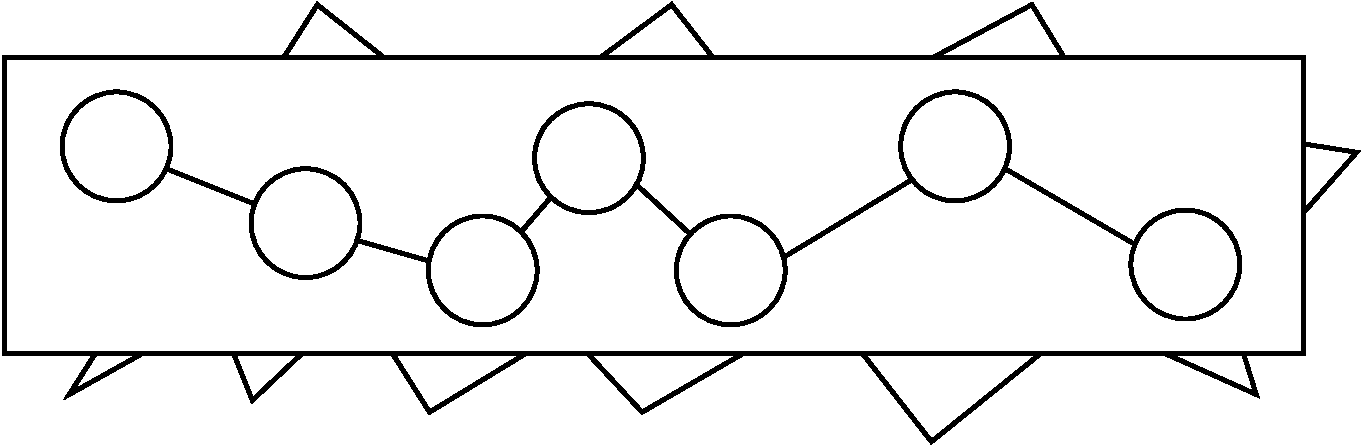
\includegraphics[width=0.9\textwidth]{test.pdf}
}
\caption{A nice caption. The larger width allows for more text without
taking too much space.}
\label{Fig2}
\end{figure*}


\section{Basic Rules for Using Latex}

First, we want to refer to the figures and the introduction.
See Figure~\ref{TUM} for the first floating figure with column width,
and Figure~\ref{Fig2} for the one using the full page width.
And here, we want to put a reference to the introduction which is
Section~\ref{introduction}.

In translating this template from German to English, I decided to
stop here. There is not really much to get from the German text
following. Anything Latex-related can also be looked up on the
net. There is a {\it huge} number of tutorials, and so on.

Please do not use to much different font sizes and styles. It should
be completely enough to go to {\em italic mode} for emphasizing something,
such as newly introduced terms.
You can refer to other parts of your paper (e.g. see 
Sec.~\ref{introduction}).
Quoting in Latex is done ``this way''.
Further, you may have problems with punctation characters.
Most of them just need to be prefixed by a backslash, for others you may
temporarily switch to math mode:
\$ \& \% \# \{ \} [ ] \_ @ \S $<$ $>$ $\backslash$ @ \textasciitilde /

Talking about math mode: you can do some very nice things this way:

\begin{equation}
a^2 + b^2 = c^2
\label{Pythagoras}
\end{equation}

Again, refering to this equation is easy (see Eq.~\ref{Pythagoras}).
If you do not need numbering for equations, use the {\em displaymath}
environment:

\begin{displaymath}
x_{1,2} = \frac{-b \pm \sqrt{b^2-4ac}}{2a}\\
\end{displaymath}

Short equations simply can be used within the regular text flow, such
as with $x \to \infty$. Obviously, math is fun with Latex.


\section{Enumerations}

Enumerations using bullet points:

\begin{itemize}
	\item this is the first item of this list of interesting facts,
	\item second item,
	\item and the last one.
\end{itemize}

They also can be numbered:

\begin{enumerate}
	\item item one,
	\item item two,
	\item item three.
\end{enumerate}

As shown, numbers always should be written out in the text, unless the
belong to a title or a formula.

\section{Literature}

At the end of your paper, you should have a nice list of used
literature. For scientific papers, this actually is needed. You always
use other works as base for your own. Usually, you are not the only
one thinking about a given difficult problem, so there is always
related work which {\em must} be cited if known to the author.

Further, if you want to copy relevant sentences from an
original paper, you {\em have} to cite them correctly, for example
in this way:

\begin{quote}
	``I think there is a world market for maybe five computers.''
	(T.J. Watson, IBM, 1943)
\end{quote}

The rest of the work (especially all the regular text) must be
written/phrased by you. If you write about some results or fact
stated in another paper, you should refer to it.
The `Analytical Engine'' --- a mechanical calculation machine ---
created by Charles Babbage in the year 1838 was based on the decimal
system
% use \cite to refer to papers from seminarpaper.bib
% this file is processed by bibtex, and it automatically adds numbering
\cite{Brom98}.

\section{Figures and Tables}

No need to understand the following text.

Figures can span either one column (see Figure~\ref{TUM}) or the full
page width (see Figure~\ref{Fig2}).
Latex automatically tries to find the best place for these floating
figures. To influence that, you may move the figure a bit to the front
of your text.
As can be seen in Figure~\ref{TUM}, using images usually results in very
bad quality. Better use vector formats: draw the figures with
{\em xfig} or {\em inkscape}, and save them as PDF. As example of
this procedure, see Figure~\ref{Fig2}).

% Narrow tables (just one column) have no * at the end
\begin{table*}

\begin{center}
% arguments:
% c = center
% l = left
% r = right (z. B. for cash)
% p = columns with fixed width, using block layout
% | = vertical line
\begin{tabular}{|l|p{2cm}|c|c|c|c|c|r|}
% horizontal line
\hline
% & means: next column
% \\ means: next row
	& Column 1 & Column 2 & Column 3 & Column 4& Column 5& Column 6& 
Amount\\
\hline
Row 1 & This column has a maximal width of 2 cm.& X & X& X& X& X& 126,00\\
\hline
Row 2 & & \multicolumn{3}{p{5cm}|}{This entry occupies three columns.}& X &X 
& 8,00\\
\hline
\multicolumn{7}{|l}{Sum} &134,00\\
\hline
\end{tabular}
\end{center}

\caption{This is the caption of the table.}
% label is for this table
\label{Tab1}

\end{table*}

Similar to figures, tables can be referred to in the text (see 
Tab.~\ref{Tab1}). However, sometimes it is useful to embed tables directly in 
the regular text flow:

\begin{center}
\begin{tabular}{|c|c|c|}
\hline
	& Column 1 & Column 2 \\
\hline
Row 1 & & \\
Row 1 & & \\
\hline
\end{tabular}
\end{center}


\section{Summary}
\label{summary}

The summary shortly repeats the core ideas and results from the
previous text. If the reader has problems understanding the summary
he knows that he should go back to the relevant sections.
Thus, the last section should consist of:

\begin{itemize}
	\item a summary,
	\item an evaluation of what was done, importance of this work,
	\item what is left, what still needs to be done,
        \item short outlook into the future.
\end{itemize}

Last but not least, we can explain anything missing yet in the evaluation
done in this paper. This allows to refer to what readers can expect from
authors in the future.

% Put citations from bibtex into References section which were not
% explicity cited.
\nocite{robotron,
stonx,vice,650sim,herculessim,zib,4004,thermal1,thermal2,rojas}


\bibliographystyle{plain}
% Literature sources are to be found in seminarpaper.bib
\bibliography{seminarpaper}
\end{document}
